\documentclass[30pt, a0paper, portrait, margin=0mm, innermargin=15mm,
               blockverticalspace=15mm, colspace=15mm, subcolspace=8mm]{tikzposter} 

% Change font     
\renewcommand{\familydefault}{\sfdefault}

\definecolor{mycol}{HTML}{326E77}
\definecolorstyle{myColorStyle}{
  \colorlet{colorOne}{darkgray}
  \colorlet{colorTwo}{gray}
  \colorlet{colorThree}{gray}
}{
  % Background Colors
  \colorlet{backgroundcolor}{colorTwo!50}
  \colorlet{framecolor}{black}
  % Title Colors
  \colorlet{titlefgcolor}{black}
  \colorlet{titlebgcolor}{colorOne}
  % Block Colors
  \colorlet{blocktitlebgcolor}{mycol}
  \colorlet{blocktitlefgcolor}{white}
  \colorlet{blockbodybgcolor}{white}
  \colorlet{blockbodyfgcolor}{black}
  % Innerblock Colors
  \colorlet{innerblocktitlebgcolor}{white}
  \colorlet{innerblocktitlefgcolor}{black}
  \colorlet{innerblockbodybgcolor}{white}
  \colorlet{innerblockbodyfgcolor}{black}
  % Note colors
  \colorlet{notefgcolor}{black}
  \colorlet{notebgcolor}{white}
  \colorlet{notefrcolor}{white}
}

% LATEX PACKAGES
% --------------
  
\usepackage{graphicx}  % package for inserting images, including .pdf
\usepackage{adjustbox} % package for cropping images
\usepackage[colorlinks=true, urlcolor=red]{hyperref} % package for url and hyperlinks
\usepackage{wrapfig}
\usepackage{lmodern} %mix italic and bold
\usepackage{hyperref}% for url
\usepackage{authblk}
\usepackage{graphicx} 
\usepackage{caption}
\usepackage{mwe}
\usepackage[absolute]{textpos}

\usepackage{graphicx}

\newcommand*\Twitter{\includegraphics[scale=0.1]{Twitter.png}}

% TITLE, AUTHORS, INSTITUTE
% -------------------------



\title{\textbf{Parasites and the eukaryotic biome - diversity is
    associated with social rank in spotted hyena}}
\author[1,2,*]{Emanuel~Heitlinger} \author[3]{Susana~C~Fereira}
\author[3]{Dagmar~Thierer} \author[3]{Heribert~Hofer}
\author[3]{Marion~L~East}

\affil[1]{\Large Research Group Ecology and Evolution of molecular Parasite-Host
  Interactions, Leibniz Institute for Zoo and Wildlife
  Research (IZW), Berlin} 
\affil[2]{\Large Department of Molecular Parasitology, Humboldt
  University (HU), Berlin}
\affil[3]{\Large Department Evolutionary Ecology, Leibniz Institute for Zoo and Wildlife
  Research (IZW), Berlin}
  \affil[*]{\textbf{Correspondence:}
  \textcolor{blue} {emanuel.heitlinger@hu-berlin.de, Heitlinger@izw-berlin.de}, \textbf{Twitter: }\textcolor{blue}{@EHeitlinger} \vspace{-6ex}}



\makeatletter
\def\maketitle{\AB@maketitle}
\makeatother

% THEME SETTING
% -------------
\usetheme{Default}
\usecolorstyle{myColorStyle}
\useblockstyle{Basic}
\usebackgroundstyle{Empty}
\usetitlestyle{Empty}


% HEAD
% ----

\begin{document}
\maketitle
\begin{columns}

% ------------------------
% COLUMN 1 ---------------
  
\column{0.5}

% Context
% ----

\block{Context, Predictions and Aims}
{
  In the spotted hyena (\textit{Crocuta crocuta}), a highly
  social, female-dominated carnivore social status
  determines access to resources.\\
  \vspace{1cm}
  \noindent
 \begin{minipage}{0.3\linewidth}                  
   \begin{left}
     \includegraphics[width=1.8\linewidth]{Hyena.png}
   \end{left}
\end{minipage}
\hfill
\begin{minipage}{0.4\linewidth}
\\Predictions:
  \begin{itemize}
 \item{High species diversity is an index of ecosystem health, the
   intestinal biome of healthier, socially dominant animals should be
   more diverse than those of subordinates.}\\
 \item{Gradual colonization of the juvenile intestine after birth
   predicts lower intestinal biome diversity in juveniles than
   adults.}
 \end{itemize}
\end{minipage} 
\hfill
\\We therefor aimed to: 
\begin{enumerate}
\item Establish an amplicon sequencing approach to assess
  intestinal eukaryotes (the eukaryome) comprehensively
\item Determine the diversity and composition of both the
  bacterial microbiome and eukaryome
\end{enumerate}
}
\block{Methods}
      {
        Study animals:
        \begin{itemize}
        \item 35 individually known adult females and 7 juveniles ($<$
          24 months) for three clans of the Serengeti ecosystem
        \item Social status categorized as above/below the median rank
        \item Parasite eggs or oocysts counted for 32 individuals
        \end{itemize}
        Amplicon sequencing
        \begin{itemize}
        \item{48 different amplicons (4 for bacterial 16S, 44 for
          eukaryote 18S) in a multi-amplicon sequencing approach}
        \item{Processed on a microfluidics PCR system (Fluidigm Access
          Array)}
        \item{Data processed using an amplified sequencing variant
          (ASV) approach provided by the R package DADA2 [1] and is
          available as an own R package [2].
        \end{itemize}
        \includegraphics[width=1\linewidth]{entropy_primers_norm_woName.png}
        \textbf{Fig 1:} Amplicons used in this study in the context of
        entropy (evolutionary conservation and information content) of
        the eukaryotic 18S gene} }
      
\block{Results: Multi-amplicon sequencing predicts coprological counts}
      {
        \begin{minipage}{0.5\linewidth}                  
          \begin{left}
            \includegraphics[scale=0.5]{Figure2_man.png}
          \end{left}
        \end{minipage}
        \hfill
        \begin{minipage}{0.5\linewidth}
          \textbf{Fig 2:} Predicting fecal egg or oocyst counts per g
          feces from the number of ASV reads. (A) Ancylostoma FEC
          vs. sequence counts for the order Rhabditida. (B)
          Diphyllobothriidae FEC vs. sequence counts for the same
          family. (C) A small size class of oocyst counts vs. added
          sequence counts for Eimeria, Isospora, Besnoitia, and
          Toxoplasma. (D) A large size class of coccidian oocysts
          vs. Eimeria sequences. All panels contain the formula for
          the specific linear model on (1+log10) transformed data, R2
          as a measure of goodness of fit, and a line representing the
          predicted relationship. The panels additionally include a
          representative micrograph depicting the egg or oocyst
          counted.\\
        \end{minipage}
        $\Rightarrow$ Quantitative assessment of eukaryotes with high
        sensitivity }

% ------------------------
% COLUMN 2 ---------------

\column{0.5}

\block{Results: Bacterial microbiome} {

  \begin{minipage}{0.5\linewidth}                  
  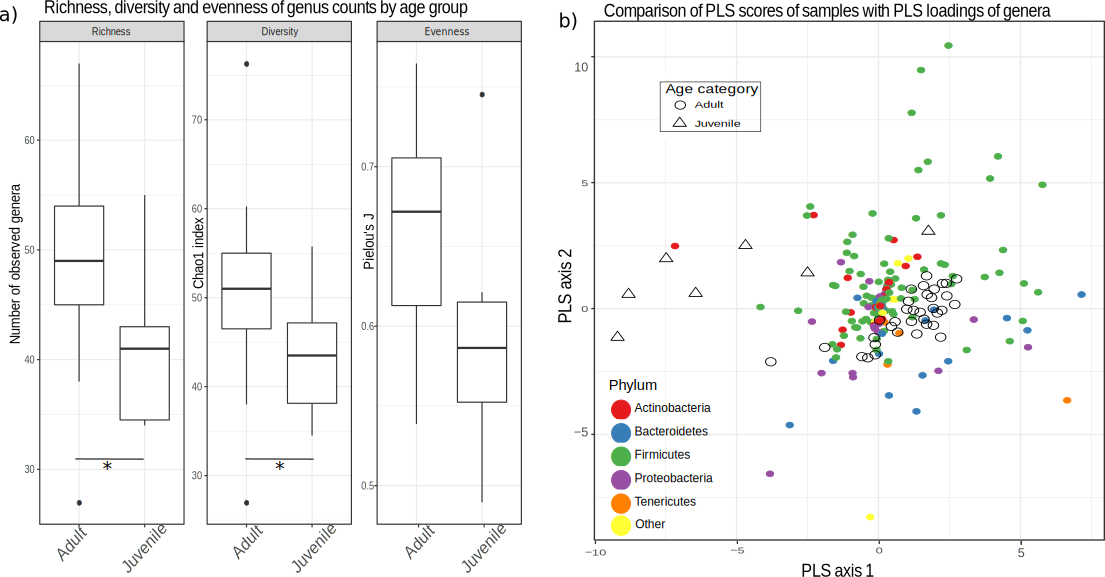
\includegraphics[scale=0.6]{Figure3_man.png} 
  \end{minipage}
  \hfill
  \begin{minipage}{0.5\linewidth}
  
    \textbf{Fig 3:} Bacterial genera richness, diversity and
    microbiome composition in different age categories. (A) Box plots
    depicting distributions observed counts of genera, diversity
    (Chao1 index) and evenness (Pielou's J) estimates on rarefied
    genera counts for juveniles and adults. $* = p < 0.05$ in exact
    Mann-Whitney U tests. (B) NMDS ordination based on pairwise
    Bray-Curtis dissimilarities partially separated juvenile from
    adult. (C) Comparison of scores (for samples) and loadings (for
    genera) from the first two axes of an optimized partial least
    squares (PLS) model, demonstrating a clear separation of adult and
    juvenile samples. Genera colored by phylum can be used to assess
    the taxa contributing (PLS loading) to the differences underlying
    this distinction.
  \end{minipage}
  (D) Log2-fold change inferred by generalized linear models for
  differences between adults and juveniles for each genus with a false
  discovery rate (FDR) $< 0.05$.  FDR is given below the dot for each
  genus color-coded for its respective phylum.

  $\Rightarrow$ Adult female hyenas have a bacterial microbiome which is more
  diverse than and differs in composition from that of juveniles.
}

\block{Results: A more diverse eukaryome in high-ranking than low-ranking hyenas} {
  \begin{minipage}{0.5\linewidth}                  
    \includegraphics[scale=0.45]{Figure4_man.png}
  \end{minipage}
  \hfill
  \begin{minipage}{0.5\linewidth}
    \testbf{Fig 5:} Eukaryome diversity and composition in high ranking
    vs. low ranking hyenas. (A) Estimates of richness, diversity and
    evenness on rarefied ASV counts for high-ranking and low-ranking
    individuals. (B) Counts for annotated ASV per genus are compared
    for high vs. low ranking hyenas. $** = p < 0.01$ based on exact
    Mann-Whitney U tests. (C) PLS scores (for samples) and PLS
    loadings (for genera) are visualized on the single PLS axis,
    demonstrating a separation of the majority of samples from
    high-ranking individuals from samples from low-ranking animals.
  \end{minipage}
  On the y-axis random scatter is introduced for visualization. The
  underlying genera are color-coded for their respective phylum.
}


\block{Summary}
{
    \includegraphics[scale=0.85]{summary.png}\\
    Green cirlcles = Results matching predictions \hspace{1cm}
    Red squares = No confirmatory results
}

\block{Funding / Misc}
{
  The study was funded by the Leibniz Institute for Zoo and
  Wildlife Research and the DFG Research Training Group 2046
  ``Parasite Infections: From Experimental Models to Natural
  Systems'' (SCF).

  \textbf{Published as:
  \hangindent=2cm  Heitlinger \textit{et al.} (2017) The
    Intestinal Eukaryotic and Bacterial Biome of Spotted Hyenas:
    The Impact of Social Status and Age on Diversity and
    Composition \textit{Front Cell Infect Microbiol. 7: 262.}}
}

% ----------

\block{References}
      {
        \begin{small}
          
          \hangindent=2cm [1] Callahan \textit{et al.} (2016) DADA2:
          High-resolution sample inference from Illumina amplicon data
          \textit{Nature Methods} 13, 581--583\\

          \hangindent=2cm [2] Heitlinger (2017). Derele/MultiAmplicon
          version 0.01 [R - package]. \textit{Zenodo} Development
          version at https://github.com/derele/MultiAmplicon
          
        \end{small}
      }


\end{columns}

% ----------------
\end{document}
\endinput
%%
%% End of file 
